% Section 7.5: where the sensors go. Figures F9, F9b, F9c; log items 56, 60, 89.
\subsection{Where the sensors go}\label{sec:paths}
\begin{notes}
\item Sensor paths over the final maps (F9: 4 shots, j30a start; F9b 2 shots, x48c; F9c 1 shot, j30b): gradient-moved sensors sweep straight lines (cosine between consecutive moves 0.52--0.75), random ones wander (about 0).
\item The design is not attracted to the unmodelled cube (share of points within 30\,mm of M1 similar to the whole scan).
\item D4: detection does not follow the distance to the nearest point nor the number of source--receiver paths (log item 89): illumination, not proximity.
\item Two- and one-shot paths: Figs.~\ref{fig:paths-2} and \ref{fig:paths-1} (Appendix~\ref{app:figures}).
\item Possibly merge into 7.2 if space is short.
\end{notes}
\begin{figure}[ht]\centering
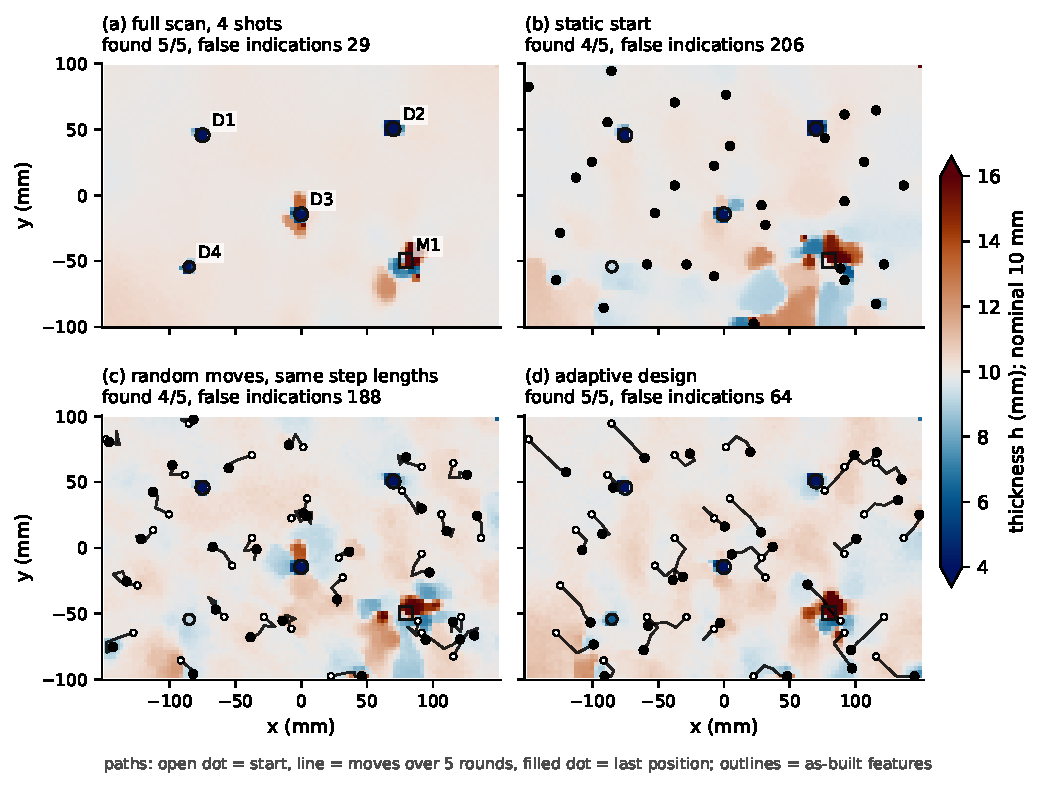
\includegraphics[width=0.9\linewidth]{F9_paths_ad_j30a.pdf}
\caption{\textbf{Where the sensors go, 4 shots} (best adaptive run, j30a start). (a) full scan, (b) static start, (c) random moves, (d) adaptive design. Adaptive sensors sweep straight lines and find D4; random moves stay near their start.}\label{fig:paths}
\end{figure}

